% !TEX encoding = UTF-8 Unicode
% !TEX TS-program = XeLaTex

\documentclass[a0,portrait]{a0poster}

\usepackage{multicol}
\columnsep=100pt 
\columnseprule=3pt 

\usepackage[svgnames]{xcolor} 

\usepackage{palatino} 

\usepackage{lipsum}

\usepackage{graphicx} % Required for including images
\graphicspath{{img/}} % Location of the graphics files
\usepackage{booktabs} % Top and bottom rules for table
\usepackage[font=small,labelfont=bf]{caption} % Required for specifying captions to tables and figures
\usepackage{amsfonts, amsmath, amsthm, amssymb} % For math fonts, symbols and environments
\usepackage{wrapfig} % Allows wrapping text around tables and figures
\usepackage{tikz}
  \usetikzlibrary{shapes,arrows}
\usepackage{float}
\usepackage{color}

\usepackage{fontspec,xltxtra,xunicode}
\defaultfontfeatures{Mapping=tex-text}
\setromanfont[Mapping=tex-text]{Fira Sans}
\setsansfont[Scale=MatchLowercase,Mapping=tex-text]{Fira Sans}
\setmonofont[]{Fira Mono}

\definecolor{supercolor}{RGB}{28,51,88}
\definecolor{nonoback}{RGB}{146,153,163}

\begin{document}

\begin{minipage}[b]{0.77\linewidth}
	\veryHuge
	\color{supercolor}
	\textbf{Ricerca, Sperimentazione e Pratica} \\%[1.1cm] % Title
\Huge\textit{nella Scuola di Musica Elettronica di Roma}\\%[1cm] % Subtitle
\huge \textbf{Giuseppe Silvi}\\%[-0.5cm] % Author(s)
\huge Conservatorio S. Cecilia di Roma\\[-0.4cm] 
\Large \texttt{me@giuseppesilvi.com}\\[0.3cm] 
\large\textit{Rapporto sui materiali di ricerca di:}\\%[2cm] % Subtitle
\huge \textbf{Elena D'Alò, Marco De Martino, Michele Papa, Claudio Panariello}\\%[0.5cm] % Author(s)
\end{minipage}
\begin{minipage}[b]{0.23\linewidth}
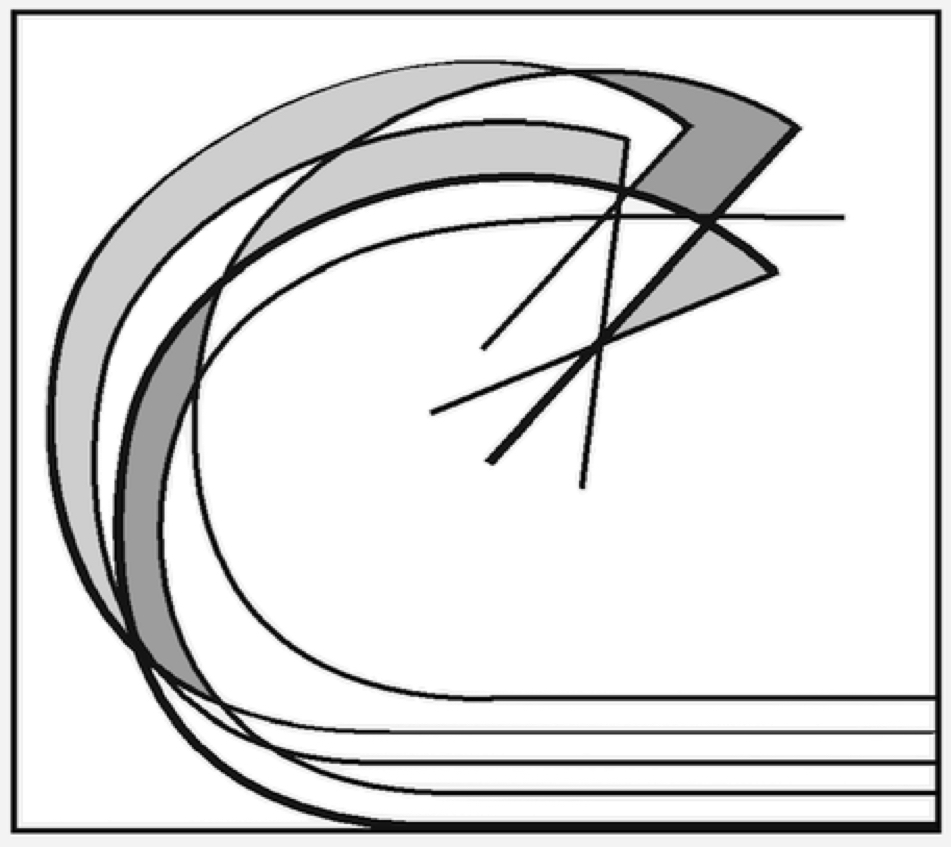
\includegraphics[width=1.\linewidth]{Conservatorio.pdf}\\
\large CONSERVATORIO S. CECILIA DI ROMA\\%[-0.4cm] 
\end{minipage}

\vspace{1cm}

\color{supercolor}

\Large
\noindent\emph{\textbf{path$\sim$}} is a Pure Data external implementing a corpus-based, concatenative analysis-resynthesis engine. Sound is acquired and resynthesised by a similarity match between audio grains, using a set of audio features extracted offline for sound corpora and in real-time for live input. 

\vfill

\normalsize

\begin{multicols}{2}

\section*{Introduction}
The basic idea of this work is offline to segment the audio files creating the grains, to perform a feature extraction analysis and to construct a k-d tree and a list of k-nearest neighbors for every grain, where every grain is represented as a set of points. In real-time, features are extracted from a live input and the most similar grain is found in the tree. Starting from this element and using its k-nn list, a pool of grains is available for the resynthesis.

\color{DarkSlateGray}

\section*{Main Objectives}
The main focus of this work is the real-time audio mosaicing. Audio mosaicing refers to the process of reconstructing the temporal evolution of a target sound from fragments taken from a source audio materials. Our interest is the application of this technique to the production of mixed contemporary composition. For this reason, we develop several functions and utilities. For example, a vectorized audio outputs control system, that allows to change, during the instantiation of the external, the number of outputs; a script-based preset management gives to the computer music designer the possibility to call different configurations and fix them in real-time thanks to a graphical editor. A debugger helps in finding errors and suggesting the possible solutions. Finally, path$\sim$ can load audio files from hard disk and from Pd's array, so analysis can be done even on on-the-fly recorded materials. \\
We are working on electronic realization with the following composers: Lara Morciano, Jos\'e Miguel Fern\'andez, Giuseppe Silvi, Daniele Pozzi.

\vspace{2cm}

\begin{figure}[H]
\centering
\begin{tikzpicture}[
	block/.style={
		node distance = 5cm,
		rectangle,
		draw,
		fill=supercolor!10,
		inner sep=5pt,
		text width=10cm,
		text badly centered,
		minimum height=2cm,
		font=\bfseries\sffamily},
	cloud/.style={
		node distance = 5cm, 
		rectangle,
		draw,
		%fill=black!10,
		inner sep=5pt,
		text width=10cm,
		text badly centered,
		minimum height=2cm,
		font=\bfseries\sffamily},	
	line/.style={
	draw,
	font=\small\sffamily}]

    % Place nodes
    \node [block] (sample) {audio samples};
    \node [block, below of=sample] (feature) {features extraction};
    \node [block, below of=feature] (database) {database};
    \node [block, below of=database] (kdtree) {k-d tree};
    \node [block, right of=kdtree,node distance=15cm] (list) {knn list};
    \node [cloud, below of=kdtree,node distance=15cm] (soutlet) {signal outputs};
    \node [cloud, right of=soutlet,node distance=15cm] (coutlet) {control outputs};	
    \node [cloud, right of=sample,node distance=15cm] (incoming) {incoming audio};
    \node [cloud, right of=feature,node distance=15cm] (rtfe) {RT features extraction};
    % Draw edges
    \path [line] (sample) -- node[left] {analysis} (feature);
    \path [line] (feature) -- node[left] {construction} (database);
    \path [line] (database) -- node[left] {sorting} (kdtree);
    \path [line,dashed] (kdtree) -- node[left]  {resynthesis} (soutlet);
    \path [line] (kdtree) -- (list);
    \path [line,dashed] (list) -- node[left, near end] {nearest neighbors} (coutlet);
    \path [line,dashed] (list) -- node[left,near start] {best match} (coutlet);
    \path [line,dashed] (incoming) -- node[left] {analysis} (rtfe);
    \path [line,dashed] (rtfe) -- node [right]{research} (kdtree);
\end{tikzpicture}
	\caption*{\color{DarkSlateGray}\textbf{\emph{path$\sim$}} structure: \newline
	white boxes and dashed lines refer to real-time operations, \newline 
	gray boxes and solid lines to offline analysis.}
\label{tikz:arch}
\end{figure}

\section*{Methods}
\subsection*{Analysis}
Two types of offline segmentations are possible; the first one is frame-based, i.e. given a frame, path$\sim$ cuts out the samples every frame and performs the analysis; the second one is onset-based, i.e. an onset detection is made and this fragmentation cares the gestural nature of audio files content. A multi-descriptors strategy is adopted: the features are mel frequency cepstral coefficients, a spectral centroid and an amplitude descriptor. Using the default parameters, the dimensionality of the feature space, i.e. dimension that every coordinate has in the feature space, is 16, 14 given by the MFCCs plus one of the spectral centroid and one of the amplitude descriptor. However, a fine tuning is possible: the mel spacing can be adjust to increase or decrease the number of coefficients and can be even deleted from all the calculations.

\subsection*{Resynthesis}
In real-time, features are extracted from a live instrument or a playback source and the most similar grain is found in the k-d tree. Starting from this grain and using its k-nn list, by default a 64 elements list, a pool of grains is available for the resynthesis. Grains can be played back deterministically following the list or choosing randomly one element from the list.

\section*{Multithreading}
\textbf{\emph{path$\sim$}} has one real-time audio thread and one worker thread, where offline analysis is performed. Using inter-thread communication and atomic synchronization, it's possible to add or change source audio materials without stopping the resynthesis. 

\section*{Results}
\subsection*{Relaxed real-time?}
Relaxed real-time is a key concept in audio mosaicing environment and the possibility to relax the real-time constraints is strongly under debate in this context. In our application, we have to distinguish the time spent in offline analysis and the latency in real-time context. \\
Our estimate about a good real-time latency limit for this task is 6 ms; even on a database size in the order of 30k, i.e. a 10 minutes audio files with a 23 ms analysis window, on authors' machine database lookups took on average less than 2 ms while offline analysis took on average less than 1 minute. However it's possible to create a queue of pre-analyzed audio files and to swap the k-d trees with the knn lists.

\section*{Conclusions}

\textbf{path$\sim$} is an open source software: it'll be released under GPLv3 and available via Deken, the Pd externals wrangler, in the stable version. \\
A high matching rate and a reasonable latency even for large database make of \textbf{path$\sim$} a good candidate for application in contemporary mixed music. The main focus of the authors was to create an extended tool for audio mosaicing for composers and computer music designers. The forthcoming researches are the requests of composers we are collaborating with; however we'll be very happy to follow new works and ideas. \\
Do you have some request? Email us or search the present author @ CIM! 

%----------------------------------------------------------------------------------------

\begin{center}\vspace{1cm}
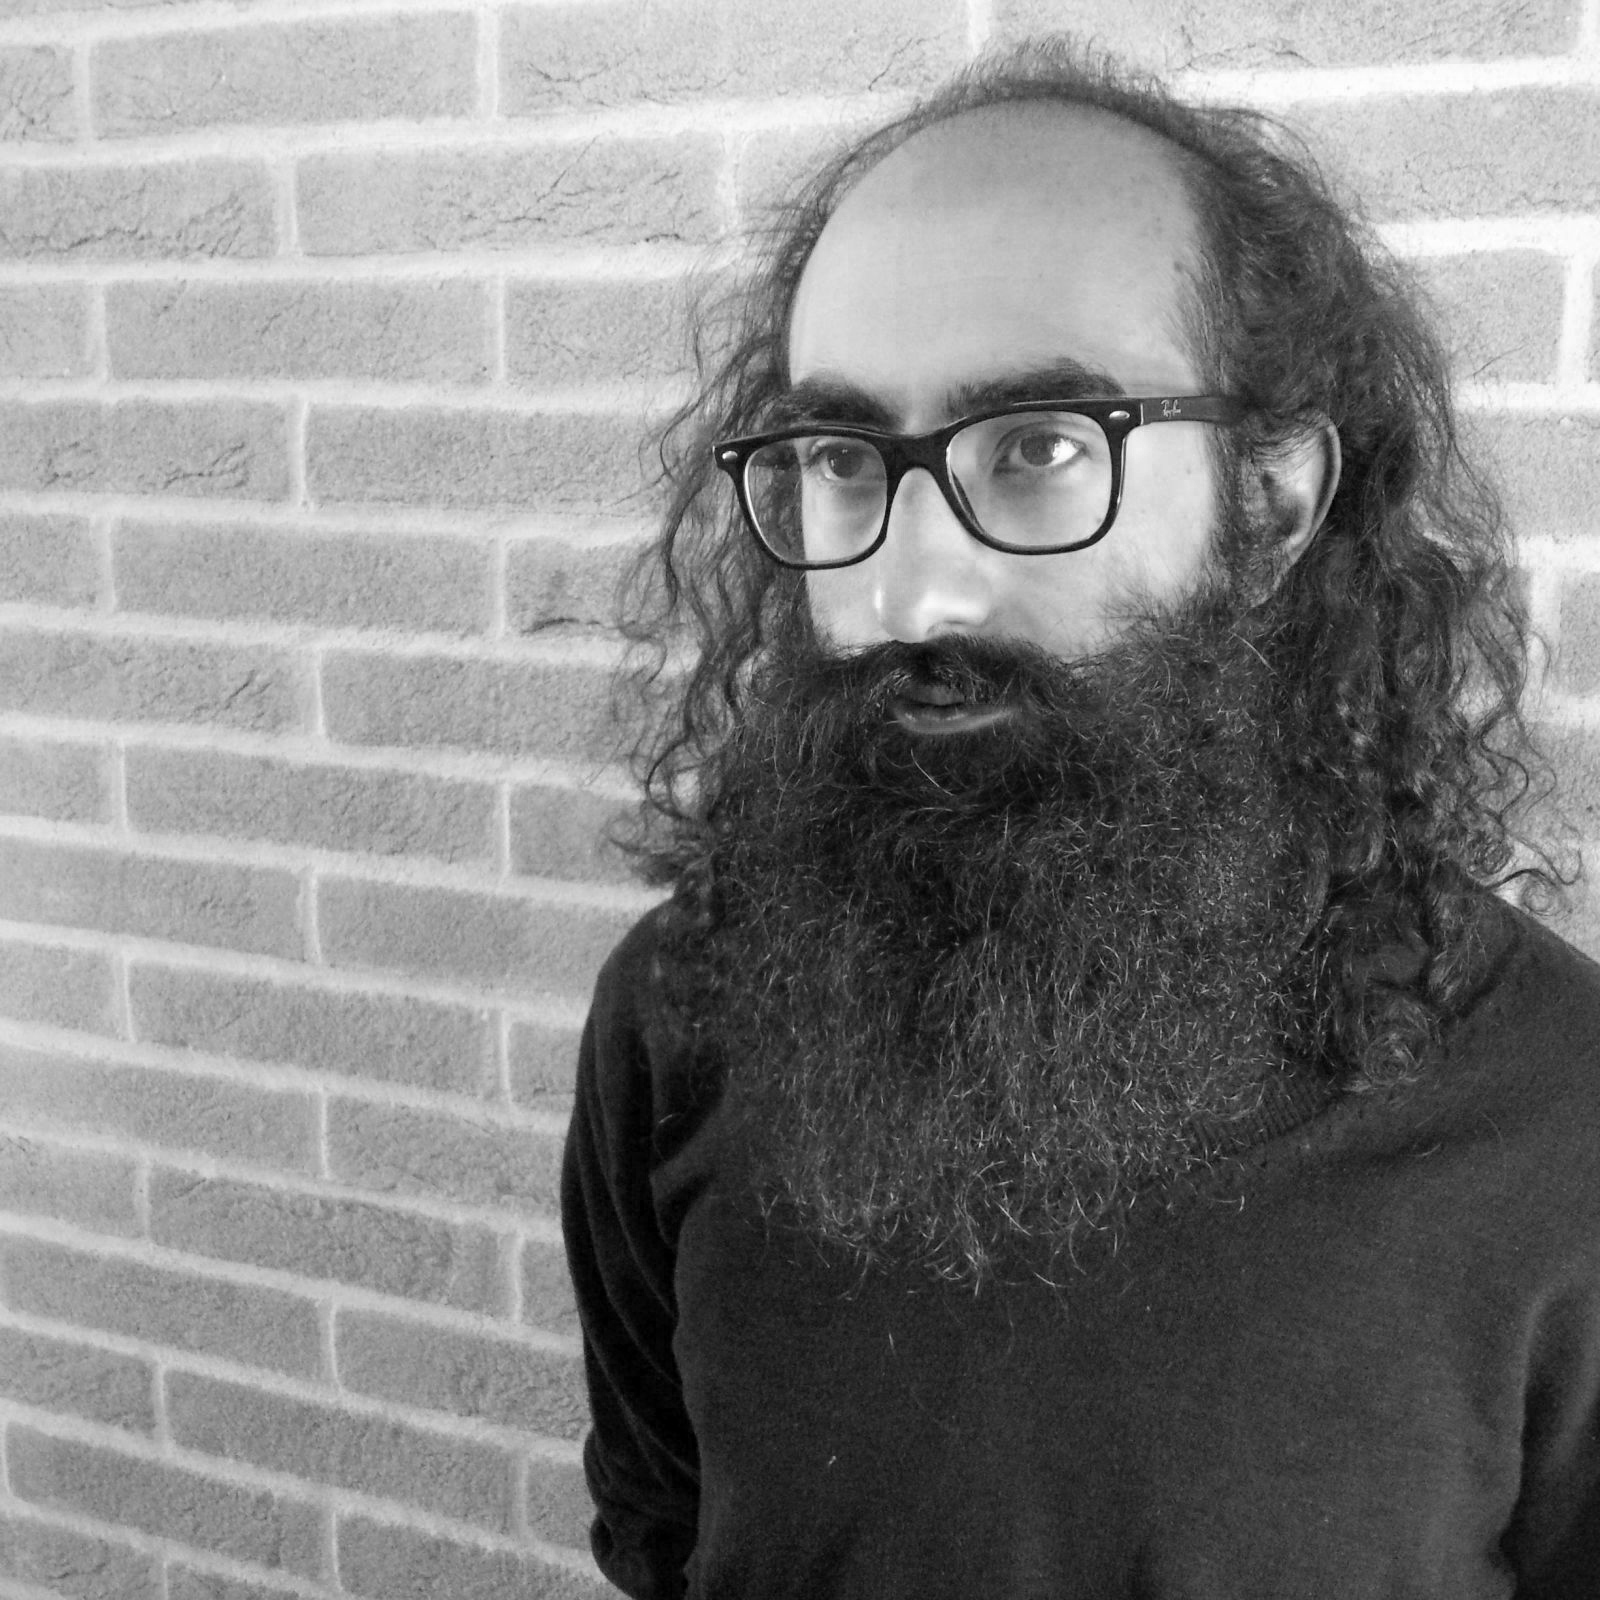
\includegraphics[width=0.99\linewidth]{mmm}
\captionof*{figure}{\textbf{Marco Matteo Markidis.} He lies here, somewhere!}
\end{center}
%\vspace{1cm}

\end{multicols}

\end{document}